%%%%%%%% MLSys submission draft: MoE prefill under ahead-of-time compilation (Cloud AI 100) %%%%%%%%

\documentclass{article}

\usepackage[T1]{fontenc}
\usepackage{microtype}
\usepackage{graphicx}
\usepackage{subfigure}
\usepackage{booktabs}
\usepackage{array}
\usepackage{amsmath}
\usepackage{amssymb}
\usepackage{xspace}
\usepackage{tikz}
\usetikzlibrary{arrows.meta,calc}
\usepackage{hyperref}

\newcommand{\theHalgorithm}{\arabic{algorithm}}

% Initial blind submission:
\usepackage{mlsys2025}
% Camera-ready: \usepackage[accepted]{mlsys2025}

\newcommand{\sys}{RankTier\xspace}
\newcommand{\naive}{$T/T$\xspace}

\mlsystitlerunning{RankTier: MoE Prefill under Ahead-of-Time Compilation}

\begin{document}

\twocolumn[
\mlsystitle{RankTier: Efficient Mixture-of-Experts Prefill on\\Ahead-of-Time Compiled Inference Accelerators}

\begin{mlsysauthorlist}
\mlsysauthor{Anonymous Authors}{anon}
\end{mlsysauthorlist}
\mlsysaffiliation{anon}{Anonymous Institution}
\mlsyscorrespondingauthor{Anonymous Authors}{anonymous@example.com}

\mlsyskeywords{Mixture of Experts, LLM Inference, Ahead-of-Time Compilation, Inference Accelerators}

\vskip 0.3in

\begin{abstract}
Mixture-of-experts (MoE) language models choose each token's experts at run time, but server inference accelerators
such as Qualcomm Cloud AI 100 execute ahead-of-time (AOT) compiled programs with static shapes and no data-dependent
control flow. The number of tokens each expert processes, its capacity, is therefore fixed at compile time, and because
some expert in some layer receives nearly every token of a prefill chunk, a program that never drops a token pads every
expert to the chunk length. The compiler's lowering of the MoE combine adds a second cost that grows with the chunk: a
dense accumulator reduced in serialized steps and rooted on one device. We present \sys, which keeps the program static
and moves the decisions it cannot compile into data. Each device ranks its experts by load at run time, binds
fixed-capacity tiers to load ranks instead of expert identities, and fetches the selected weights through an index gather
that the compiler lowers to indirect DMA; a token-owned combine then lets each device sum only its own tokens' expert
rows before one distributed cross-device sum. On Qwen3-30B-A3B across the four SoCs of a Cloud AI 100 Ultra card, with
the KV cache on device, \sys prefills 128-, 256- and 512-token chunks 4.05$\times$, 2.45$\times$ and 2.94$\times$ faster
than the production compilation, without dropping a token in any measured prompt. Against a baseline with the same
compilation settings but the compiler's combine and every expert padded to the chunk length, the reduction redesign alone
is 2.06--2.38$\times$ faster, while the rank-bound tiers pay only on top of it, adding 1.06--1.37$\times$.
\end{abstract}
]

\printAffiliationsAndNotice{}

%-----------------------------------------------------------------------------------------------------------------------
\section{Introduction}
\label{sec:intro}

Mixture-of-experts (MoE) layers let a language model grow its parameter count without a matching growth in per-token
compute: a router sends each token to a few of many experts, and only those experts run
\citep{shazeer2017outrageously,fedus2022switch}. Recent open models use MoE layers throughout; Qwen3-30B-A3B routes each
token to 8 of 128 experts in each of its 48 layers and activates 3.3B of its 30.5B parameters \citep{yang2025qwen3}, and
Mixtral and DeepSeek-V3 follow the same pattern \citep{jiang2024mixtral,deepseek2024v3}. During prefill, a serving system
processes the prompt in chunks of $T$ tokens \citep{agrawal2024sarathi}, so each MoE layer sees $8T$ token-to-expert
assignments whose distribution over experts is known only after its router runs. GPU systems absorb this variation with
kernels that accept data-dependent shapes: block-sparse GEMMs that never drop a token \citep{gale2023megablocks},
parallelism and pipelining chosen at run time \citep{hwang2023tutel}, and all-to-all exchanges sized per batch
\citep{rajbhandari2022deepspeedmoe}.

Server inference accelerators take a different path. Qualcomm Cloud AI 100 \citep{chatha2021qualcomm}, like
XLA-compiled TPU programs \citep{lepikhin2021gshard} and the statically scheduled Groq TSP \citep{abts2020tsp}, runs a
model as a program compiled ahead of time: tensor shapes, the partition of every operator over cores and devices, and the
schedule are fixed before the first request, and on Cloud AI 100 the compiler rejects control flow that depends on data.
Static planning is what lets the compiler orchestrate 16 cores per SoC and four SoCs per card, but for MoE it turns two
run-time quantities into compile-time constants: how many token rows each expert computes, and how expert outputs flow
back to their tokens. Both grow costly at long chunks, which prefill uses to amortize weight traffic, and they have two
structural consequences.

\textbf{(i) Padding sized by the worst chunk.} Each expert occupies a lane of fixed capacity, and every lane computes its
full capacity however few tokens it receives. Routing is skewed and workload-dependent: in our routing captures, one expert in
some layer receives 256 of 256 and 508 of 512 tokens, and the experts most loaded in one workload are rarely the most
loaded in another (\S\ref{sec:mot-pad}). A program that never drops a token therefore pads all 128 experts to
$T$, 16$\times$ the routed assignments. Calibrated per-expert capacities do not escape this: fitted to 200 prompts from
all eight workloads, they still overflow on 12--36\% of each workload's held-out prompts, and they converge on $T$.

\textbf{(ii) Reductions shaped by the compiler rather than by the tokens.} By default the partitioner slices each
expert's down projection across the four SoCs, which costs 121.6\,MiB of cross-SoC traffic per layer, and it returns
expert outputs to tokens through a dense accumulator per stage that is zero-filled, updated between stages, reduced in
serialized steps and summed across SoCs on a single SoC, spilling to DRAM from $T=256$ on. Even with the slicing removed
and the worst serialization rewritten, this combine path takes 51\%, 64\% and 68\% of an MoE layer at $T=128$, 256 and
512 in the production MXFP6 precision (\S\ref{sec:mot-red}). Expert-parallel compilation alone makes the full model 46\%
faster at $T=128$ but 11--12.5\% slower than production at 256 and 512 tokens, because the dense combine grows with $T$.

We present \sys, a design for MoE prefill that keeps the program static and moves the decisions the compiler cannot make
into data. It rests on one property of the compiler: a program cannot branch on data, but it can address by data. A
weight gather indexed by a run-time tensor is lowered to indirect weight DMA and runs as fast as a static weight stream
(\S\ref{sec:mot-addr}). \sys therefore fixes lanes and capacities at compile time and decides at run time which
expert each lane serves. Each SoC counts the tokens routed to its 32 experts, sorts them, and gives the expert of rank
$r$ a lane in the tier that covers $r$. Capacities bound to ranks can be small because the order statistics of per-SoC
load are stable across workloads even when expert identities are not: over 200 held-out prompts of eight workloads, the
16th most loaded expert of a SoC never received more than 12 of 128 tokens, while a fixed expert order needs up to
84--127 rows at \emph{every} position (Figure~\ref{fig:rank}). Three tiers of 8, 8 and 16 lanes per SoC fit the
compiler's even core mapping and its sequential stages. For the reduction, \sys compiles every expert whole on one SoC,
restores the on-device KV cache that this setting breaks by making attention head-parallel, and lets each SoC own its
tokens: it gathers only the rows of each token's experts that live on the SoC, sums them locally, and leaves one
elementwise cross-SoC sum that the compiler distributes as a reduce-scatter.

We implement \sys as graph transformations of the exported model and evaluate the full 48-layer Qwen3-30B-A3B with MXFP6
expert weights on the four SoCs of one Cloud AI 100 Ultra card, with the KV cache retained on device. \sys prefills 128-,
256- and 512-token chunks in 122, 206 and 356\,ms, 4.05$\times$, 2.45$\times$ and 2.94$\times$ faster than the
production compilation. An ablation against a naive baseline that keeps the compiler's combine and capacity $T$ shows
how the two parts interact: the reduction redesign alone gives 2.06--2.38$\times$, the padding series alone at most
1.05$\times$, and the padding series on top of the reduction redesign another 1.06--1.37$\times$. No lane exceeded its capacity in any measured prompt, and the error against an FP32
reference stays at the level of the production program.

The paper makes three contributions:
\begin{itemize}
\item A characterization of MoE prefill on an AOT-compiled multi-SoC accelerator, which identifies compile-time capacity
  and compiler-shaped reductions as the two costs that grow with the chunk, and establishes which run-time mechanisms the
  compiler does and does not offer (\S\ref{sec:mot}).
\item \sys: rank-bound tiered capacities built from run-time sorting and index-gathered weights, and a token-owned
  reduction on expert-parallel compilation with an on-device KV cache, all expressed as static graphs that the compiler
  maps evenly (\S\ref{sec:design}--\ref{sec:impl}).
\item An end-to-end evaluation on the full model at three chunk lengths: a step-by-step ladder, a 2$\times$2 ablation of
  the two optimization series, and the negative results that bound the design space (\S\ref{sec:eval}).
\end{itemize}

%-----------------------------------------------------------------------------------------------------------------------
\section{Background and Related Work}
\label{sec:bg}

\subsection{MoE Inference}

An MoE layer replaces the feed-forward block with $E$ experts and a router. For a token with hidden state
$x_t\in\mathbb{R}^d$, the router selects the set $\mathcal{K}_t$ of $k$ experts with the largest gate values and returns
\begin{equation}
y_t=\sum_{e\in\mathcal{K}_t} w_{t,e}\,W^{\mathrm{down}}_e\big(\mathrm{SiLU}(W^{\mathrm{gate}}_e x_t)\odot W^{\mathrm{up}}_e x_t\big),
\label{eq:moe}
\end{equation}
with normalized gate weights $w_{t,e}$. Qwen3-30B-A3B uses $E=128$, $k=8$, $d=2048$ and an expert width of 768, so an
expert's three matrices hold 9\,MiB in FP16. Implementations group assignments by expert, run each expert's GEMMs over
its gathered token rows, and return the weighted rows to their tokens; under expert parallelism the experts are spread
over devices and dispatch and combine become cross-device exchanges \citep{lepikhin2021gshard,rajbhandari2022deepspeedmoe}.
Training systems bound each expert's work by a capacity factor and drop the tokens beyond it
\citep{lepikhin2021gshard,fedus2022switch}; at inference, a dropped assignment changes the model's output. Prefill
processes the prompt in chunks of $T$ tokens and writes their keys and values to the KV cache; decode then generates one
token per step \citep{kwon2023vllm,agrawal2024sarathi}. A chunk gives each layer $8T$ assignments, $2T$ per SoC on average
when four SoCs hold 32 experts each.

\subsection{MoE Systems}

GPU systems handle the data-dependent shape of expert work directly. MegaBlocks expresses expert computation as
block-sparse GEMMs and never drops tokens \citep{gale2023megablocks}; Tutel switches parallelism and pipelining at run
time \citep{hwang2023tutel}; DeepSpeed-MoE and FasterMoE optimize expert-parallel inference and training around the
all-to-all exchange \citep{rajbhandari2022deepspeedmoe,he2022fastermoe}; Lina schedules all-to-all traffic and expert
resources dynamically \citep{li2023lina}. Placement studies exploit routing structure: ExFlow uses inter-layer expert
affinity to cut all-to-all traffic \citep{yao2024exflow}, and \citet{yu2025patterns} profile data movement across
workloads to derive a prefill-aware expert placement. \citet{huang2024toward} characterize MoE inference and replace
static capacity with dynamic gating; Pre-gated MoE predicts the next layer's experts to overlap their loading
\citep{hwang2024pregated}. Expert-choice routing gives every expert a fixed number of tokens by construction
\citep{zhou2022expertchoice}, which removes the padding problem but changes the model. Closest to our setting, DynaMoE
recompiles a static-shape program when capacities change during training \citep{kossmann2022dynamoe}. On our
accelerator a full-model program takes 6--23 minutes to compile, so capacities cannot follow each chunk by recompilation,
and none of the GPU mechanisms above exists in a program without data-dependent shapes.

\subsection{AOT-Compiled Inference Accelerators}

A Cloud AI 100 SoC has 16 AI cores and four 64-bit LPDDR4x channels with 136\,GB/s and up to 32\,GB
\citep{chatha2021qualcomm,qualcomm2025arch}. Each core combines a scalar VLIW processor, a vector unit and a tensor unit
with 4K FP16 MACs, and holds an 8\,MB software-managed vector memory and a 1\,MB L2 cache. The Ultra card used here
carries four SoCs, 64 cores in total, under a shared 150\,W board limit.

The compiler takes an ONNX graph and one shape specialization per chunk length and produces a static program. It
partitions each operator over the 16 cores of a SoC and, by multi-device tensor slicing, over the SoCs; the degree of
weight splitting across SoCs is a compile option. Matrix weights can be stored as MXFP6 \citep{rouhani2023mx}, which the
vector unit dequantizes while the tensor unit computes. A KV cache stays on device when the compiler can pair each cache
input with its updated output (\emph{retained state}); otherwise the cache becomes host I/O. Control flow must be
static: an ONNX \texttt{If} with a non-constant condition is rejected at compile time. Dynamic-shape compilers for CPUs
and GPUs handle such workloads with shape functions and run-time dispatch \citep{shen2021nimble,zhu2021disc}; the
accelerator programs considered here have no such runtime.

%-----------------------------------------------------------------------------------------------------------------------
\section{Motivation}
\label{sec:mot}

We study the MoE layers of Qwen3-30B-A3B compiled for the four SoCs of one Cloud AI 100 Ultra card (setup in
\S\ref{sec:setup}). The exported graph \citep{qefficient} runs a layer's 128 experts as two stages of 64 \emph{lanes}; a
lane is one expert's gate, up and down GEMMs over a fixed number of gathered token rows, its capacity $C$. The production
program uses $C=T$ in both stages, the only capacity that can never drop a token. Three observations motivate \sys:
capacities attached to experts must cover the worst chunk, the compiler's combine grows with the chunk, and the compiler
nevertheless lets a program address weights by data.

\subsection{Capacities Attached to Experts Cover the Worst Chunk}
\label{sec:mot-pad}

Without data-dependent control flow a lane cannot skip rows: every lane of a compiled stage computes its full capacity of
$C$ rows, however few tokens it receives. Capacity is work, and the question is which capacities a program may use
without dropping tokens.

We captured the routing of all 48 layers for 50 prompts of 128 tokens from each of eight workloads, GSM8K, MMLU,
SWE-bench Lite issues, HumanEval and its JavaScript version, Alpaca instructions, CNN/DailyMail articles and Chinese XNLI
sentence pairs \citep{cobbe2021gsm8k,hendrycks2021mmlu,jimenez2024swebench,chen2021humaneval,muennighoff2024octopack,taori2023alpaca,hermann2015cnndm,conneau2018xnli},
and for chunks of 256 and 512 tokens from four of them (Appendix~\ref{app:calib}), with the model's FP32 layers on the
CPU. The load is skewed: in some layer one expert receives 127 of 128, 256 of 256 and 508 of 512 tokens. The skew is
also workload-specific: across workloads the 16 most loaded experts of a layer agree with a Jaccard index of 0.00--0.33,
against 0.52--0.88 between the two halves of one workload, and the 64 most loaded agree at 0.29--0.70 (HumanEval and its
JavaScript version, which share their problem statements, are the exception).

\begin{figure}[t]
\centering
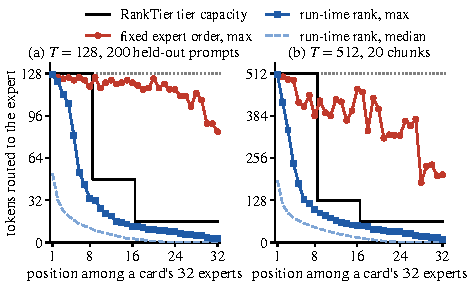
\includegraphics[width=\columnwidth]{figures/fig_rank_identity.pdf}
\vskip -0.08in
\caption{Rows a SoC must reserve for its expert at each position, as the largest load observed there. Red: experts in a
fixed order, ranked by their mean load on calibration prompts (a: the first half of each workload's prompts, evaluated on
the other half; b: leave-one-out over the chunks). Blue: experts ordered at run time by their load in the chunk itself. Black: the tier
capacities \sys uses. Dotted: capacity $T$.}
\label{fig:rank}
\vskip -0.1in
\end{figure}

A program that attaches capacities to experts, fixing which lane serves which expert, must reserve at each lane the
largest load that its expert can receive. Figure~\ref{fig:rank} shows the cost. Ordering each SoC's 32 experts by their
mean load on calibration prompts and reading the held-out loads at each position of that order, the maximum is 84--127 of
128 rows at every position at $T=128$: a drop-free fixed layout needs 91\% of the rows of padding everything to $T$
(73\% at $T=512$). Fitting stage capacities to calibration data does not rescue a fixed layout: with hot and cold stages
fitted to 200 prompts from all eight workloads, 12--36\% of each workload's held-out prompts still overflow in some layer,
and the fitted capacities approach the chunk length, 122 and 105 of 128 rows in the median layer.

Padding is not free once $T$ grows. In a one-layer replay, the tensor-unit time of a SoC's 16 most loaded experts is 44,
310 and 921\,\textmu s per core at capacities 92, 158 and 296, a 21$\times$ increase for 3.2$\times$ the rows, while their
weight stream stays constant. In an instrumented profile of the full model at $T=512$, the stage that holds each SoC's 16 most
loaded experts at capacity $T$ takes a quarter of every layer (2.35 of 9.24\,ms), and even after the reduction redesign
of \S\ref{sec:red}, capacity-$T$ padding makes latency grow in proportion to the chunk (131.7, 258.9 and 498.4\,ms at
$T=128$, 256 and 512; Table~\ref{tab:ladder}), so a longer chunk gains nothing per token.

\subsection{The Compiler's Combine Grows with the Chunk}
\label{sec:mot-red}

The combine of Eq.~(\ref{eq:moe}), expert rows back to their tokens, is where the compiler's defaults cost most.

\textbf{Slicing across SoCs.} With its default heuristic the partitioner splits the down-projection weights of all 64
lanes four ways along the output dimension, so each SoC computes a 512-column slice of every expert's output. This
requires an all-gather of the intermediate activation (36\,MiB per stage at $C=128$) and a re-shard of the output
(24\,MiB per stage) before the combine; cross-SoC traffic reaches 121.6\,MiB per layer, while gate and up projections stay
expert-parallel.

\textbf{A dense accumulator.} The exported combine scatters each stage's weighted expert rows into an accumulator of
shape $[64, T, d]$, zero-filled by a single core, gathered and updated between the two stages, reduced over each SoC's
16 lanes by one einsum that the compiler runs through DRAM on one core, and finally summed over the four SoCs on four
cores of SoC~0. From $T=256$ on, this last sum also spills into a DRAM-backed reduction on one core (0.84\,ms). Every
part scales with $T$; none scales with the number of routed rows.

\begin{table}[t]
\caption{Device time of one MoE layer with the dense combine, split into the combine path (the accumulator's gap
between the stages and SoC~0's reduction tail) and everything else. MXFP6, expert-parallel compilation and the
dense-path rewrites of \S\ref{sec:red}, one-layer replays with stage capacities fitted to the input, instrumented.}
\label{tab:combine}
\vskip 0.1in
\begin{center}
\begin{small}
\begin{tabular}{@{}rrrrr@{}}
\toprule
$T$ & Layer, ms & Combine path, ms & Rest, ms & Share \\
\midrule
128 & 2.34 & 1.19 & 1.15 & 51\% \\
256 & 4.35 & 2.78 & 1.57 & 64\% \\
512 & 8.62 & 5.84 & 2.78 & 68\% \\
\bottomrule
\end{tabular}
\end{small}
\end{center}
\vskip -0.15in
\end{table}

Table~\ref{tab:combine} measures the combine path after expert-parallel compilation and after the rewrites of
\S\ref{sec:red}, which remove its most serialized parts: it still takes 51\% of an MoE layer at $T=128$ and 68\% at 512.
On the full model, compiling experts whole on each SoC with the KV cache kept on device (\S\ref{sec:ep}) reduces prefill
latency from 494.6 to 267.1\,ms at $T=128$ but increases it from 505.3 to 568.6\,ms at 256 and from 1049.1 to
1164.1\,ms at 512 (Table~\ref{tab:ladder}), because its dense combine grows with $T$.

\subsection{A Static Program Can Address by Data}
\label{sec:mot-addr}

What the compiler withholds is control flow; what it offers is indexing. We probed three mechanisms on one-layer replays
and two-layer cuts of the full model.

\textbf{Index-gathered weights are free.} Replacing the three weight constants of a layer's first stage by
\texttt{Gather(bank, idx)}, with the 64-entry index arriving at run time, leaves the layer at 2.796\,ms, the same as with
static weights, and the output is bit-identical: the compiler lowers the gather to an indirect weight DMA that reads the
MXFP6 bytes directly. Only this form stays fast. Per-SoC constants and batched gathers run 2.3--3.7$\times$ slower,
because the compiler either keeps their weights in FP16 or spreads per-SoC MatMuls over all SoCs, and the one gathered
constant is replicated on every SoC. A configuration with
one partition per SoC stores each bank once, but the runtime then executes the SoCs one after another, 1.7$\times$ slower
for a single inference.

\textbf{Lane counts must divide 16.} The compiler maps a stage onto a SoC's cores by its number of lanes per SoC. With a
lane count that divides 16 (we tested 2, 4, 8 and 16) the mapping is balanced; with 17--19 lanes it splits the GEMMs unevenly (3 to 36
tensor-unit operations per core), and from 20 lanes on it packs the whole stage onto four cores per SoC, which takes
3.7--4.3\,ms for a stage that runs in 0.5\,ms on 16 cores.

\textbf{Stages run one after another.} The compiler schedules a layer's expert stages sequentially, in its own order;
in our tiered programs a stage of $L$ lanes per SoC ran one lane per core on $L$ cores. Every additional stage adds a
window of its own.

These properties define the space \sys works in: fixed lanes whose experts are chosen by index at run time, tier widths
from $\{1,2,4,8,16\}$ lanes per SoC, and as few stages as the padding allows.

%-----------------------------------------------------------------------------------------------------------------------
\section{\sys}
\label{sec:design}

Section~\ref{sec:mot} leads to three requirements. First, capacity must follow each chunk's load without control flow,
so the program must choose at run time which expert a lane serves and bind capacities to a quantity that is stable across
chunks. Second, the reduction must scale with the routed rows rather than with lanes $\times\,T$, and no SoC may root it.
Third, every mechanism must be a static graph that the compiler maps evenly: lane counts from $\{1,2,4,8,16\}$ per SoC,
one gathered constant per weight, and few stages.

\begin{figure*}[t]
\centering
% Figure: one MoE layer under RankTier. Bars: sorted token counts of SoC 2 in layer 20 of the held-out 512-token chunk.
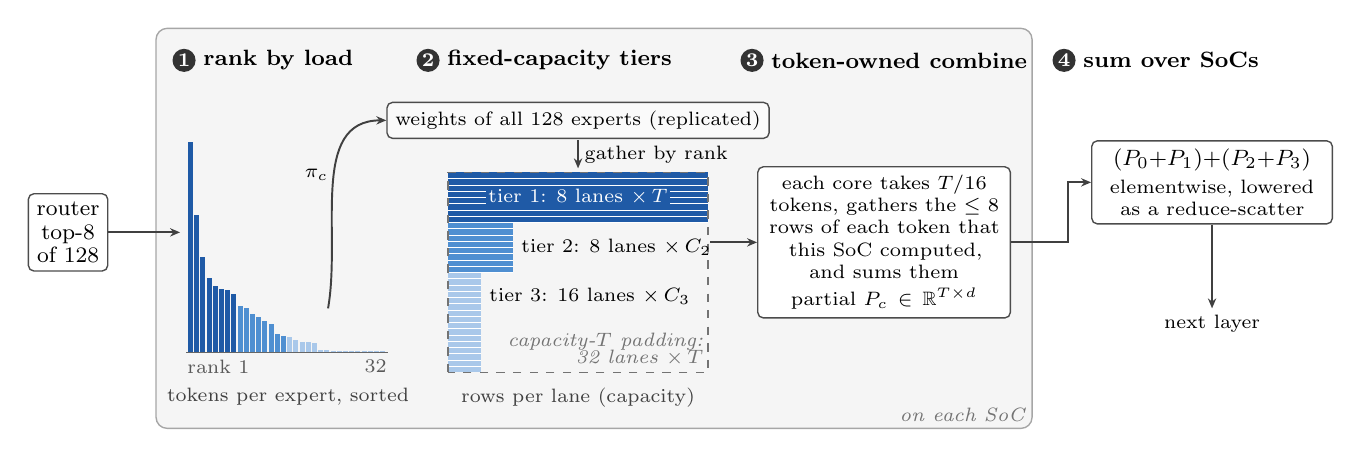
\begin{tikzpicture}[x=1in, y=1in, font=\footnotesize, >={Stealth[length=3.6pt, width=3pt]},
  box/.style={draw=black!70, rounded corners=2pt, align=center, inner sep=3pt, fill=white, line width=0.5pt},
  flow/.style={->, line width=0.7pt, draw=black!75},
  num/.style={circle, fill=black!80, text=white, inner sep=0.7pt, font=\scriptsize\bfseries},
  head/.style={anchor=west, font=\footnotesize\bfseries, inner sep=1pt}]
\definecolor{tierA}{RGB}{31,90,166}\definecolor{tierB}{RGB}{79,143,209}\definecolor{tierC}{RGB}{169,200,234}
% frame for the per-SoC steps 1-3
\draw[rounded corners=4pt, fill=black!4, draw=black!35, line width=0.5pt] (0.74,0.02) rectangle (5.12,2.02);
\node[anchor=south east, font=\scriptsize\itshape, text=black!55, inner sep=1pt] at (5.10,0.04) {on each SoC};
% router
\node[box] (router) at (0.30,1.00) {router\\[-1pt]top-8\\[-1pt]of 128};
\draw[flow] (router.east) -- (0.86,1.00);
% ---- (1) rank the SoC's 32 experts
\node[num] at (0.88,1.86) {1}; \node[head] at (0.96,1.86) {rank by load};
\foreach [count=\i] \c in {176,115,80,62,56,53,52,49,39,37,32,30,26,24,15,14,13,10,9,9,8,2,2,1,1,0,0,0,0,0,0,0} {
  \pgfmathsetmacro{\x}{0.90 + (\i-1)*0.031}
  \pgfmathsetmacro{\h}{max(0.006, \c/176*1.05)}
  \ifnum\i<9 \def\col{tierA}\else\ifnum\i<17 \def\col{tierB}\else\def\col{tierC}\fi\fi
  \fill[\col] (\x,0.40) rectangle ++(0.025,\h);
}
\draw[black!60, line width=0.4pt] (0.89,0.40) -- (1.90,0.40);
\node[anchor=north west, font=\scriptsize, text=black!65, inner sep=1pt] at (0.88,0.38) {rank 1};
\node[anchor=north east, font=\scriptsize, text=black!65, inner sep=1pt] at (1.91,0.38) {32};
\node[anchor=north, font=\scriptsize, align=center, text=black!75, inner sep=1pt] at (1.40,0.24) {tokens per expert, sorted};
% ---- (2) tiers; weights gathered by rank
\node[num] at (2.10,1.86) {2}; \node[head] at (2.18,1.86) {fixed-capacity tiers};
\node[box, minimum width=1.30in, fill=black!2, font=\scriptsize] (bank) at (2.85,1.56) {weights of all 128 experts (replicated)};
\draw[flow] (1.60,0.62) to[out=80, in=180] node[pos=0.55, left, font=\scriptsize, inner sep=2pt] {$\pi_c$} (bank.west);
\draw[flow] (2.85,1.46) -- node[right, font=\scriptsize, inner sep=2pt] {gather by rank} (2.85,1.32);
\def\L{0.03125}
\fill[tierA] (2.20,1.05) rectangle (3.50,1.30);
\fill[tierB] (2.20,0.80) rectangle (2.525,1.05);
\fill[tierC] (2.20,0.30) rectangle (2.3625,0.80);
\foreach \k in {1,...,31} {\draw[white, line width=0.25pt] (2.20,{0.30+\k*\L}) -- ({\k>23 ? 3.50 : (\k>15 ? 2.525 : 2.3625)},{0.30+\k*\L});}
\draw[dashed, black!55, line width=0.5pt] (2.20,0.30) rectangle (3.50,1.30);
\node[fill=tierA, text=white, font=\scriptsize, inner sep=1pt] at (2.85,1.175) {tier 1: 8 lanes $\times\,T$};
\node[anchor=west, font=\scriptsize, inner sep=1pt] at (2.55,0.925) {tier 2: 8 lanes $\times\,C_2$};
\node[anchor=west, font=\scriptsize, inner sep=1pt] at (2.39,0.68) {tier 3: 16 lanes $\times\,C_3$};
\node[anchor=south east, font=\scriptsize\itshape, text=black!55, align=right, inner sep=1.5pt] at (3.50,0.31) {capacity-$T$ padding:\\[-2pt]32 lanes $\times\,T$};
\node[anchor=north, font=\scriptsize, text=black!75, inner sep=1pt] at (2.85,0.24) {rows per lane (capacity)};
% ---- (3) token-owned combine
\node[num] at (3.72,1.86) {3}; \node[head] at (3.80,1.86) {token-owned combine};
\node[box, text width=1.18in, font=\scriptsize] (comb) at (4.38,0.95) {each core takes $T/16$ tokens, gathers the $\le 8$ rows of each token that this SoC computed, and sums them\\[2pt] partial $P_c\in\mathbb{R}^{T\times d}$};
\draw[flow] (3.51,0.95) -- (comb.west);
% ---- (4) sum over SoCs
\node[num] at (5.28,1.86) {4}; \node[head] at (5.36,1.86) {sum over SoCs};
\node[box, text width=1.12in, font=\scriptsize] (sum) at (6.02,1.25) {{\footnotesize $(P_0{+}P_1){+}(P_2{+}P_3)$}\\[2pt] elementwise, lowered as a reduce-scatter};
\draw[flow] (comb.east) -- (5.30,0.95) |- (sum.west);
\draw[flow] (sum.south) -- (6.02,0.62) node[below, font=\scriptsize, inner sep=2pt] {next layer};
\end{tikzpicture}

\vskip -0.05in
\caption{One MoE layer under \sys. (1) Each SoC counts the tokens routed to its 32 experts and sorts them (bars: SoC~2 in
layer 20 of the held-out 512-token chunk; colors mark the tiers). (2) Three tiers of lanes with compile-time capacities
($C_2=128$, $C_3=64$ at $T=512$) serve the experts by rank; their weights are gathered from a bank of all 128 experts
through the rank permutation $\pi_c$. The filled area is the padded work, against the dashed capacity-$T$ layout.
(3) Each core gathers and sums the rows of its own tokens. (4) One elementwise sum over SoCs completes the layer.}
\label{fig:overview}
\vskip -0.1in
\end{figure*}

Figure~\ref{fig:overview} shows one MoE layer under \sys. \S\ref{sec:ep} describes the compilation setting that makes
experts local, \S\ref{sec:red} the reduction, \S\ref{sec:sort} the run-time ranking and \S\ref{sec:tiers} the tiers.

\subsection{Expert-Parallel Compilation with an On-Device KV Cache}
\label{sec:ep}

We compile with a weight-splitting degree of one across SoCs (\texttt{-mdts-mos=1}), which forbids cutting any weight
matrix across SoCs. The lane axis is then the only way to distribute the batched expert GEMMs, and each SoC computes 16
whole experts per stage, one per core; the all-gather and re-shard of the down projection disappear, and the layer's
cross-SoC traffic falls from 121.6 to 1.5\,MiB.

The setting is global and also stops the compiler from splitting the attention projections by KV head. The cache update
then comes out token-sliced while its input is whole, the compiler cannot pair the 96 cache inputs with their outputs,
and all 192 KV buffers become host I/O. We restore the pairing at the graph level with \emph{head-parallel attention}:
the four KV-head groups of eight query heads each \citep{ainslie2023gqa} become a leading batch axis of every attention
operator, with per-group weights of shapes $[4,2048,1024]$ for queries, $[4,2048,128]$ for keys and values and
$[4,1024,2048]$ for the output projection, whose four partial outputs are summed at the end. Under expert-parallel
compilation the batch axis lands one group per SoC, the cache operations of KV head $h$ stay on SoC $h$, and the program
again exposes no KV buffer. On a two-layer cut the head-parallel program runs in 12.5\,ms of device time against 23.3\,ms
for the production setting, with 30 instead of 265\,MiB of cross-SoC traffic. The regrouped output projection changes the
FP16 summation order; on two layers the logits differ from the production program by $6.8\times10^{-4}$ relative $L_2$,
with the same argmax.

\subsection{Token-Owned Reduction}
\label{sec:red}

The reduction is rebuilt in three steps. Each keeps the model's arithmetic and changes only where and in which order the
sums run.

\textbf{Dense-path rewrites.} Three rewrites remove serialized work that the export introduces. (i) The first stage's
outputs were added to rows gathered from the freshly zeroed accumulator; we drop this read of zeros. (ii) The per-SoC sum
over lanes, one einsum that the compiler ran through DRAM on one core, is cut into 16 tiles of $T/16$ tokens. (iii) The
routing's prefix sums over tokens, which give each assignment its row in the expert's compact input and ran as a serial
\texttt{CumSum} on one core, become Hillis--Steele scans of $\log_2 T$ shift-and-add steps \citep{hillis1986data}. All
three leave the output bit-identical.

\textbf{Token-owned combine.} The dense accumulator exists because the export combines by lane, scattering each lane's
rows to their tokens. \sys combines by token (Algorithm~\ref{alg:combine}). The router's top-$k$ output already lists each
token's experts; with integer arithmetic on the lane layout and the per-expert slot tables that the routing computes
anyway, every (token, $j$) pair maps to the stage and row of the SoC's compact expert outputs that hold its result, or to
a masked sentinel when the expert lives on another SoC. One gather per stage then fetches at most eight rows per token;
masking, the addition of the stages and a sum over the rows give the SoC's $[T,d]$ partial output. Each core owns a tile
of $T/16$ tokens, so the per-SoC combine needs no cross-core traffic.

\begin{algorithm}[t]
\caption{Token-owned combine on SoC $c$}
\label{alg:combine}
\begin{algorithmic}[1]
\REQUIRE top-$k$ experts $\mathcal{K}[t,1..k]$ of each token $t$; lane map $\ell(e)\mapsto(s,c',l)$ (stage or tier, SoC, lane);
  $\mathrm{slot}[e,t]$, row of token $t$ in expert $e$'s input; weighted outputs $O_s\in\mathbb{R}^{L_sC_s\times d}$ of SoC $c$
\FOR{all $t\le T$, $j\le k$ \textbf{in parallel}}
  \STATE $e\leftarrow\mathcal{K}[t,j]$;\; $(s,c',l)\leftarrow\ell(e)$
  \IF{$c'=c$}
    \STATE $\mathit{idx}_s[t,j]\leftarrow l\,C_s+\mathrm{slot}[e,t]$;\; $m_s[t,j]\leftarrow1$
  \ELSE
    \STATE $\mathit{idx}_s[t,j]\leftarrow0$;\; $m_s[t,j]\leftarrow0$ \COMMENT{masked}
  \ENDIF
\ENDFOR
\FOR{each core $q$, owning tokens $t\in$ tile $q$}
  \STATE $P_c[t]\leftarrow\sum_s\sum_{j}m_s[t,j]\,O_s[\mathit{idx}_s[t,j]]$ \COMMENT{$\le k$ rows}
\ENDFOR
\STATE $y\leftarrow(P_0+P_1)+(P_2+P_3)$ \COMMENT{elementwise, over SoCs}
\end{algorithmic}
\end{algorithm}

Two lowering details matter. The device gather does not zero-fill out-of-range indices, so the safe index and the
explicit mask are both required. And the per-SoC work must stay on the lane axis that the compiler already splits over
SoCs: written as explicit per-SoC slices, the combine made the compiler distribute its tiles over SoCs and ship expert
outputs between them, raising cross-SoC traffic from 3 to 78\,MiB and the layer's device time from 4.3 to 8.6\,ms.

\textbf{Elementwise final sum.} The remaining sum over the four partials was written as 16 einsum tiles, which the
compiler lowers to a reduction template on four cores per SoC. Written as the elementwise tree $(P_0+P_1)+(P_2+P_3)$ per
token tile, the additions spread over all 16 cores of each SoC. In the full model the compiler lowers this sum as a
reduce-scatter: each SoC adds a quarter of the tokens, and the next layer's input normalization, which runs split by
token rows, gathers the rest. No SoC receives all four partials.

\subsection{Run-Time Rank Sort}
\label{sec:sort}

Each SoC owns a fixed quarter of the 128 experts. After the router, \sys counts each expert's tokens from the routing
mask and sorts each SoC's 32 counts (a \texttt{TopK}), which gives a per-SoC permutation $\pi_c$ from rank to expert.
Lane $j$ of the tier starting at rank $a_i$ serves the expert of rank $a_i+j$; its three weight matrices come from
\texttt{Gather(bank,$\,\pi$)} on one constant that holds all 128 experts, lowered to indirect DMA (\S\ref{sec:mot-addr}).

Two choices keep the sort off the critical path. First, the routing mask, the prefix scans and the slot tables are
computed once over all 128 experts in native order, independent of the sort; only a row permutation of these tables and
the weight gathers wait for it. Sorting first and running the routing on permuted columns makes everything wait
(12 layers: +2.5\,ms over capacity-$T$ padding, against +1.6\,ms). Second, gathered weights are sensitive to the compiler's
maximum tile size: with the default, the first expert GEMM waits 0.085\,ms for its first gathered tile, with 512\,KiB
tiles 0.032\,ms. The best size is 512\,KiB for $T\le256$ and 1024\,KiB for $T=512$ (\S\ref{sec:eval-pad}).

The price is memory. The gathered constant is replicated, so every SoC holds the weights of all 128 experts,
22.5\,GiB per SoC instead of 6.7\,GiB, within the SoC's 32\,GB. The program also returns every lane's token count in
every layer, so an overflow, a rank that received more tokens than its tier's capacity, is detectable after each chunk.

\subsection{Tiered Capacities}
\label{sec:tiers}

A tier is a stage of $L_i$ lanes per SoC at capacity $C_i$ that covers ranks $a_i,\dots,a_i+L_i-1$, with
$\sum_iL_i=32$. Every expert keeps exactly one lane, so tiers change only the padding: the same experts compute the same
tokens, and the output is bit-identical to the two-tier sort. A SoC computes $\sum_iL_iC_i$ rows per layer, against $32T$
with capacity-$T$ padding.

\textbf{Capacities from order statistics.} The first tier has capacity $T$, since rank 1 can receive every token. For
$i>1$, $C_i$ is the largest load observed at rank $a_i$, the tier's first rank, over calibration chunks, times a headroom
$h=1.28$, rounded up to a multiple of 16 and capped at $T$; since ranks are sorted, rank $a_i$ bounds the whole tier. We
calibrate on routing captures of the eight workloads: the 128-token prompts of \S\ref{sec:mot-pad}, 56 chunks of 256
tokens and 20 of 512. Order statistics are predictable for a structural reason: if a SoC receives $n_c$ assignments in a
chunk, its $r$-th most loaded expert holds at most $n_c/r$ of them, and $n_c$ is a sum over 32 experts, $2T$ on average and
at most 1.9$\times$ that in our 256- and 512-token captures. An expert-bound capacity must instead cover the worst case of one expert, which
is $T$.

\textbf{Choosing the tiers.} Rows alone favor many tiers: under our calibration three stages need 65--67\% of the rows of
a two-tier split at $T$ and $T/8$, four stages 52--58\% and five 48--56\%. But stages run sequentially and each adds a
window of its own, so the design balances rows against stages. At $T=512$ the first tier is bound by the SoC's shared
memory traffic rather than by per-core compute: eight lanes of 512 rows finish in 0.8--1.0\,ms, sixteen lanes in 2.2\,ms,
although each core does the same work. \sys uses three tiers of 8, 8 and 16 lanes per SoC (Table~\ref{tab:tiers}),
12--13$T$ rows per SoC against $18T$ for two tiers and $32T$ for capacity-$T$ padding; \S\ref{sec:eval-pad} shows that a
fourth tier costs more than it saves.

\begin{table}[t]
\caption{Tier designs, lanes per SoC $\times$ capacity, and the padded rows each SoC computes per layer.}
\label{tab:tiers}
\vskip 0.1in
\begin{center}
\begin{small}
\setlength{\tabcolsep}{4pt}
\begin{tabular}{@{}rccccc@{}}
\toprule
$T$ & Ranks 1--8 & 9--16 & 17--32 & Rows & vs.\ two tiers / \naive \\
\midrule
128 & 8$\times$128 & 8$\times$48 & 16$\times$16 & 13$T$ & 72\% / 41\% \\
256 & 8$\times$256 & 8$\times$64 & 16$\times$32 & 12$T$ & 67\% / 38\% \\
512 & 8$\times$512 & 8$\times$128 & 16$\times$64 & 12$T$ & 67\% / 38\% \\
\bottomrule
\end{tabular}
\end{small}
\end{center}
\vskip -0.15in
\end{table}

%-----------------------------------------------------------------------------------------------------------------------
\section{Implementation}
\label{sec:impl}

\sys is a set of ONNX graph transformations, about 1,100 lines of Python, applied to the Qwen3-30B-A3B graph that the
vendor's QEfficient library exports for Cloud AI 100 \citep{qefficient}. Each step of \S\ref{sec:design} is a separate
pass, so every intermediate program can be compiled and measured. The passes locate operators by structure rather than
by name (layer 0 numbers some nodes differently and folds a 64-lane constant into its stage), regenerate the
$T$-dependent constants of the scans and tiles for each chunk length, and clone the stage subgraph once per tier with its
own row order, weight gathers and capacity. A static \texttt{If} in the export that squeezes the token table is replaced
by the equivalent \texttt{Squeeze} in every clone, and the combine's map from a lane to (tier, SoC, row) becomes a set of
small per-tier tables. For the ablation (\S\ref{sec:eval-abl}) the same pass can instead feed the export's own combine.

Each chunk length is its own program, with sequence length $T$ and context $2T$. We compile with MXFP6 matrix weights,
FP16 activations, 16 cores per SoC, depth-first scheduling, expert-parallel slicing and retained state
(Appendix~\ref{app:flags}). Static programs compile in 6--12 minutes and occupy 25\,GB; programs with gathered weights
compile in 12--23 minutes and occupy 88\,GB, because the program file keeps an FP16 copy of each gathered bank.

%-----------------------------------------------------------------------------------------------------------------------
\section{Evaluation}
\label{sec:eval}

We ask how much \sys speeds up the full model (\S\ref{sec:eval-e2e}), what each part of the reduction and of the padding
design contributes (\S\ref{sec:eval-red}, \S\ref{sec:eval-pad}), whether the output is preserved (\S\ref{sec:eval-acc}),
and which alternatives failed (\S\ref{sec:eval-neg}).

\subsection{Experimental Setup}
\label{sec:setup}

\textbf{Hardware and model.} One Cloud AI 100 Ultra card, four SoCs with 16 cores and 32\,GB each, platform SDK 1.21.6.
Qwen3-30B-A3B, all 48 layers, batch 1, MXFP6 matrix weights and FP16 activations as in the production deployment. Every
program keeps its KV cache on device.

\textbf{Programs.} Seven programs, each adding one step to the one before it (Table~\ref{tab:ladder}): (1) the production
compilation of the exported graph, with default partitioning, the dense combine and capacity $T$ in both stages;
(2)~expert-parallel compilation with head-parallel attention, which keeps the export's combine and capacity $T$ and is
our \emph{naive \naive} baseline; (3) the dense-path rewrites; (4) the token-owned combine; (5) the elementwise final sum;
(6) the run-time rank sort with two tiers at $T$ and $T/8$; (7) \sys's three tiers.

\textbf{Prompts.} At $T=128$ the first chunk of a GSM8K chat prompt; at 256 and 512 held-out chunks built from GSM8K
test questions outside the calibration range. Latency depends on a chunk only through its routing, and on a single layer
it varied by about 1\% across 200 prompts of four workloads.

\textbf{Protocol.} Host latency of one chunk, the median of three rounds of 20 inferences after warm-up. All programs of
one chunk length run back to back in one session, with anchor programs repeated before and after; steps 6 and 7 ran in a
second session and are chained to the first through step 5, which ran in both and agreed within 0.13\%. Rounds agree
within 0.6\%. For accuracy we compare the last-position logits with an FP32 CPU run of the same chunk, check the
next-token prediction, and read back every lane's token count.

\subsection{End-to-End Results}
\label{sec:eval-e2e}

\begin{table}[t]
\caption{Prefill latency of one chunk (ms) for the seven programs, and the change against the program above it.}
\label{tab:ladder}
\vskip 0.1in
\begin{center}
\begin{small}
\setlength{\tabcolsep}{2.5pt}
\begin{tabular}{@{}lr@{\,}lr@{\,}lr@{\,}l@{}}
\toprule
Program & \multicolumn{2}{c}{$T=128$} & \multicolumn{2}{c}{$T=256$} & \multicolumn{2}{c}{$T=512$} \\
\midrule
1 Production          & 494.6 &  & 505.3 &  & 1049.1 &  \\
2 + expert/head par.  & 267.1 & {\scriptsize $-$46.0\%} & 568.6 & {\scriptsize $+$12.5\%} & 1164.1 & {\scriptsize $+$11.0\%} \\
3 + rewrites          & 158.4 & {\scriptsize $-$40.7\%} & 355.9 & {\scriptsize $-$37.4\%} & 729.1 & {\scriptsize $-$37.4\%} \\
4 + token-owned       & 131.7 & {\scriptsize $-$16.9\%} & 258.9 & {\scriptsize $-$27.3\%} & 498.4 & {\scriptsize $-$31.6\%} \\
5 + elementwise sum   & 129.5 & {\scriptsize $-$1.6\%} & 252.1 & {\scriptsize $-$2.6\%} & 491.1 & {\scriptsize $-$1.5\%} \\
6 + rank sort         & 126.3 & {\scriptsize $-$2.5\%} & 215.2 & {\scriptsize $-$14.6\%} & 421.6 & {\scriptsize $-$14.2\%} \\
7 + tiers (\sys)      & \textbf{122.2} & {\scriptsize $-$3.2\%} & \textbf{206.2} & {\scriptsize $-$4.2\%} & \textbf{356.3} & {\scriptsize $-$15.5\%} \\
\midrule
Reductions, 2$\to$5  & \multicolumn{2}{c}{2.06$\times$} & \multicolumn{2}{c}{2.26$\times$} & \multicolumn{2}{c}{2.37$\times$} \\
Padding, 5$\to$7     & \multicolumn{2}{c}{1.06$\times$} & \multicolumn{2}{c}{1.22$\times$} & \multicolumn{2}{c}{1.38$\times$} \\
vs.\ naive \naive, 2$\to$7 & \multicolumn{2}{c}{2.19$\times$} & \multicolumn{2}{c}{2.76$\times$} & \multicolumn{2}{c}{3.27$\times$} \\
vs.\ production     & \multicolumn{2}{c}{\textbf{4.05$\times$}} & \multicolumn{2}{c}{\textbf{2.45$\times$}} & \multicolumn{2}{c}{\textbf{2.94$\times$}} \\
Tokens/s, 1 / 7     & \multicolumn{2}{c}{259 / 1047} & \multicolumn{2}{c}{507 / 1241} & \multicolumn{2}{c}{488 / 1437} \\
\bottomrule
\end{tabular}
\end{small}
\end{center}
\vskip -0.15in
\end{table}

\begin{figure}[t]
\centering
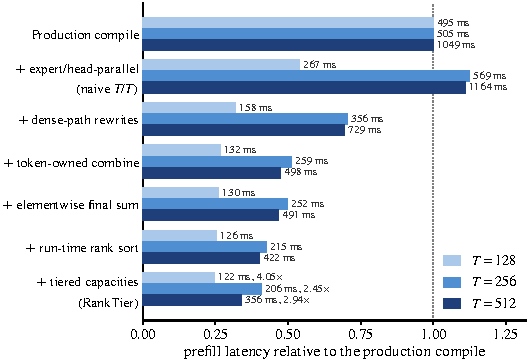
\includegraphics[width=\columnwidth]{figures/fig_ladder.pdf}
\vskip -0.08in
\caption{Prefill latency of the seven programs relative to the production compilation at the same chunk length, with
the latency of each program and the speedup of \sys.}
\label{fig:ladder}
\vskip -0.1in
\end{figure}

Table~\ref{tab:ladder} and Figure~\ref{fig:ladder} give the results. \sys prefills 128-, 256- and 512-token chunks in
122.2, 206.2 and 356.3\,ms, 4.05$\times$, 2.45$\times$ and 2.94$\times$ faster than the production compilation, and
2.19$\times$, 2.76$\times$ and 3.27$\times$ faster than naive \naive. In the order of the ladder, the reduction steps
contribute 2.06--2.37$\times$ and the padding steps after them 1.06--1.38$\times$, both growing with $T$; \S\ref{sec:eval-abl}
separates the two series. Only with both does a longer chunk pay: per-token latency falls from 0.95 to 0.70\,ms between
$T=128$ and 512 under \sys, stays at 0.97--1.03\,ms with the token-owned combine at capacity $T$, and rises from 2.09
to 2.27\,ms under naive \naive.

\subsection{Ablation of the Two Series}
\label{sec:eval-abl}

\begin{table}[t]
\caption{The two series alone and together on the full model: prefill latency per chunk (ms) and speedups over naive
\naive (N). One session per chunk length, each program timed twice in mirrored order; P$_2$ ran in a second session,
chained through N and P.}
\label{tab:ablation}
\vskip 0.1in
\begin{center}
\begin{small}
\setlength{\tabcolsep}{3pt}
\begin{tabular}{@{}lllrrr@{}}
\toprule
 & Reduction & Padding & $T=128$ & $T=256$ & $T=512$ \\
\midrule
N & export & \naive & 267.3 & 569.9 & 1162.2 \\
R & ours & \naive & 129.6 & 253.2 & 488.7 \\
P$_2$ & export & rank sort & 267.4 & 551.3 & 1110.3 \\
P & export & sort, tiers & 388.4 & 669.7 & 1379.3 \\
D & ours & sort, tiers & \textbf{122.6} & \textbf{206.8} & \textbf{355.8} \\
\midrule
\multicolumn{3}{@{}l}{Reduction alone, N/R} & 2.06$\times$ & 2.25$\times$ & 2.38$\times$ \\
\multicolumn{3}{@{}l}{Rank sort alone, N/P$_2$} & 1.00$\times$ & 1.03$\times$ & 1.05$\times$ \\
\multicolumn{3}{@{}l}{Sort and tiers alone, N/P} & 0.69$\times$ & 0.85$\times$ & 0.84$\times$ \\
\multicolumn{3}{@{}l}{Padding after the reduction, R/D} & 1.06$\times$ & 1.22$\times$ & 1.37$\times$ \\
\multicolumn{3}{@{}l}{Both (\sys), N/D} & \textbf{2.18$\times$} & \textbf{2.76$\times$} & \textbf{3.27$\times$} \\
\bottomrule
\end{tabular}
\end{small}
\end{center}
\vskip -0.15in
\end{table}

The ladder adds the reduction steps before the padding steps, so it cannot show what each series gives alone.
Table~\ref{tab:ablation} starts both from naive \naive and adds programs that apply only the padding series: the rank
sort and the tiers feeding the export's own combine. The export's scatter writes only into an accumulator with as many
lanes as the stage, so tiers of equal width share one accumulator, read-modify-written as the export's second stage is,
and tiers of 8, 8 and 16 lanes per SoC need two accumulators, of 32 and 64 lanes, where the two-tier sort needs one.

The reduction series alone gives 2.06--2.38$\times$. The padding series alone gives almost nothing: the rank sort
1.00--1.05$\times$, and with the three tiers the program runs at only 0.69--0.85$\times$ the baseline's speed. The same padding series
gives 1.06--1.37$\times$ once the reduction series is in place. Two effects explain the difference. First, padding
shortens only the expert stages, while most of the naive layer is combine work that grows with lanes$\,\times\,T$
(Table~\ref{tab:combine}): the 2.8\,ms per layer that padding saves at $T=512$ is 27\% of the reduced layer, and the
same saving would be only 11\% of the 24.2\,ms naive layer. Second, under the export's combine the tiers cost
accumulators: the second accumulator adds a zero fill and a lane reduction through DRAM, and the third tier costs 2.5,
2.5 and 5.6\,ms per layer at $T=128$, 256 and 512 (not profiled). In the token-owned combine, a tier adds only one gather of at most eight rows per
token. The reduction redesign is therefore a prerequisite for the padding series, not an independent gain.

\subsection{Reduction}
\label{sec:eval-red}

\textbf{Expert parallelism alone is not enough.} Step 2 removes the down projection's slicing and is 46\% faster than
production at $T=128$. At 256 and 512 tokens it is 12.5\% and 11.0\% slower, because the dense
combine that remains grows with $T$ (Table~\ref{tab:combine}); the head-parallel attention in this step only restores the
on-device cache.

\textbf{The rewrites and the token-owned combine carry the reduction.} The dense-path rewrites save 37--41\% at every
chunk length and the token-owned combine another 16.9\%, 27.3\% and 31.6\%, growing with $T$ as the accumulator it removes does.
The mechanism is visible on one layer in isolation: with the same fitted capacities, the token-owned layer runs in 2.19,
3.23 and 5.69\,ms at $T=128$, 256 and 512 against 2.61, 5.30 and 9.93\,ms for the dense combine; at $T=256$ the work
after the last expert stage falls from 2.0\,ms to under 0.1\,ms per SoC plus the cross-SoC sum. The elementwise final
sum adds 1.5--2.6\%.

\textbf{What remains is small.} In a two-layer profile at $T=512$, the MoE partial sums exchanged between SoCs are 6\,MiB
and 0.30--0.34\,ms per layer, 14\% of the cross-SoC bytes, and the tail from the last expert GEMM to the completed sum
is 0.48\,ms. Removing the exchange entirely would save about 3\% of the model. For this reason we did not pursue
placements that make tokens SoC-local (\S\ref{sec:eval-neg}).

\subsection{Padding}
\label{sec:eval-pad}

\textbf{The rank sort pays from 256 tokens on.} With two tiers at $T$ and $T/8$, step 6 saves 2.5\% at $T=128$, where the
expert stages stream weights at their bandwidth floor and the cold stage's 112 fewer rows per lane hide under that stream,
and 14.6\% and 14.2\% at 256 and 512. The sort adds a dependency on every layer's critical path, router to sort to weight
gathers; with the tile sizes below it costs less than it saves even at $T=128$.

\begin{figure}[t]
\centering
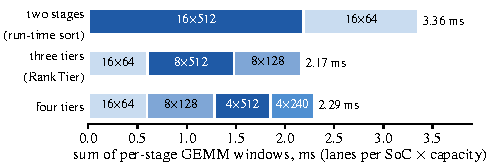
\includegraphics[width=\columnwidth]{figures/fig_stages.pdf}
\vskip -0.08in
\caption{GEMM window of each expert stage in execution order at $T=512$, two-layer profiles; segments are the per-stage
medians over SoCs, labeled with lanes per SoC $\times$ capacity.}
\label{fig:stages}
\vskip -0.1in
\end{figure}

\textbf{Three tiers, not more.} Step 7 saves another 3.2\%, 4.2\% and 15.5\%. Figure~\ref{fig:stages} shows why three tiers
are the right number at $T=512$. With two tiers, the 16 lanes at capacity 512 take 2.2\,ms per layer; split into eight
lanes at 512 and eight at 128, the same ranks take 0.8--1.0 and 0.65--0.72\,ms, although each core of the eight-lane
stage does the same work as before, because the stage is bound by the SoC's memory traffic. A fourth tier removes more
rows but adds a sequential window: on two layers, four tiers are 8.6\% faster than two, three tiers 14.1\%. At $T=256$ the
extra stage's window absorbs most of the saving (Table~\ref{tab:ladder}).

\begin{table}[t]
\caption{Rank sort on 12-layer cuts: latency change against the token-owned program at capacity $T$ (default tiles)
for three maximum tile sizes.}
\label{tab:tiles}
\vskip 0.1in
\begin{center}
\begin{small}
\begin{tabular}{@{}rrrr@{}}
\toprule
$T$ & Default tiles & 512\,KiB & 1024\,KiB \\
\midrule
128 & $+4.7\%$ & $\mathbf{-1.4\%}$ & -- \\
256 & $-5.1\%$ & $\mathbf{-18.2\%}$ & $-7.9\%$ \\
512 & $-12.7\%$ & $-9.3\%$ & $\mathbf{-15.9\%}$ \\
\bottomrule
\end{tabular}
\end{small}
\end{center}
\vskip -0.15in
\end{table}

\textbf{Tile size.} Table~\ref{tab:tiles} shows the sensitivity of gathered weights to the compiler's maximum tile size.
With default tiles the rank sort is 4.7\% slower than the token-owned program at capacity $T$ at $T=128$; with 512\,KiB
tiles it is 1.4\% faster. The
best size moves with the chunk, 512\,KiB up to 256 tokens and 1024\,KiB at 512; static weights prefer the default, which
small tiles slow by 1--2\%. Each program therefore uses its own best size.

\textbf{Capacity usage.} The largest lane loads observed in the timed chunks were 122, 20 and 8 of capacities 128, 48 and
16 at $T=128$; 251, 36 and 17 of 256, 64 and 32 at 256; and 508, 83 and 37 of 512, 128 and 64 at 512. The first tier is
nearly full in every case, which is why its capacity stays at $T$: taking each layer's calibration maximum instead would
remove 10--15\% of its rows but overflow in one and five layers of the held-out chunks.

\subsection{Accuracy}
\label{sec:eval-acc}

\begin{table}[t]
\caption{Relative $L_2$ error of the last-position logits against FP32, and the next token (\checkmark: matches FP32).}
\label{tab:acc}
\vskip 0.1in
\begin{center}
\begin{small}
\setlength{\tabcolsep}{4pt}
\begin{tabular}{@{}lccc@{}}
\toprule
Program & $T=128$ & $T=256$ & $T=512$ \\
\midrule
1 Production                 & 0.188 \checkmark & 0.089 $\times$ & 0.095 \checkmark \\
2--3 Naive \naive, rewrites & 0.172 \checkmark & 0.077 \checkmark & 0.094 \checkmark \\
4 Token-owned combine     & 0.172 \checkmark & 0.073 \checkmark & 0.092 \checkmark \\
5 Elementwise sum            & 0.190 \checkmark & 0.077 \checkmark & 0.095 \checkmark \\
6--7 Rank sort, \sys         & 0.170 \checkmark & 0.087 $\times$ & 0.088 \checkmark \\
\bottomrule
\end{tabular}
\end{small}
\end{center}
\vskip -0.15in
\end{table}

Every program stays at the error level of the production program's MXFP6 weights (Table~\ref{tab:acc}). The programs
differ from production, and from one another, only in FP16 summation order: head-parallel attention regroups the output
projection, which alone moves 343 of 49,152 routing assignments at $T=128$, and the token-owned combine sums a token's
rows in a different order; neither leaves that level. Tiers are bit-identical to the two-tier sort, since
the same experts compute the same tokens. The next token matches FP32 in every case except the 256-token chunk, whose two
leading FP32 logits are 0.58 apart; production and the rank-sorted programs pick the second. No lane exceeded its
capacity in any program.

\subsection{What Did Not Work}
\label{sec:eval-neg}

\begin{table}[t]
\caption{Alternatives we built or analyzed and rejected ($T=512$ unless noted).}
\label{tab:neg}
\vskip 0.1in
\begin{center}
\begin{footnotesize}
\setlength{\tabcolsep}{3pt}
\begin{tabular}{@{}>{\raggedright\arraybackslash}p{0.33\columnwidth}>{\raggedright\arraybackslash}p{0.25\columnwidth}>{\raggedright\arraybackslash}p{0.36\columnwidth}@{}}
\toprule
Alternative & Result & Reason \\
\midrule
Sort first, then route on permuted columns & $+$2.5 vs.\ $+$1.6\,ms (12 layers, $T{=}128$) & all routing waits for the sort \\
Row-chunked expert GEMMs & $+$25\%, $+$66\% (one layer) & each chunk re-streams and re-dequantizes the weights \\
One partition per SoC & 1.7$\times$ slower & the runtime runs partitions in sequence \\
Per-layer first-tier capacity & $-$10--15\% of its rows & held-out chunks overflow in 1--5 layers \\
Co-locate experts that fire together & 3.63$\to$2.42 SoCs per token & doubles lower-tier loads; the exchange is 3\% \\
Split first-tier experts over two lanes & $+$6\% (two layers) & 16 lanes stay on 8 cores; 1.8$\times$ dequantization \\
Four tiers & $-$8.6\% vs.\ $-$14.1\% & one more sequential window \\
No depth-first scheduling & $+$1--2\% & stages still run in sequence \\
\bottomrule
\end{tabular}
\end{footnotesize}
\end{center}
\vskip -0.15in
\end{table}

Table~\ref{tab:neg} lists the alternatives we rejected. Two are instructive. Splitting a heavily loaded expert over
several lanes, each with a chunk of its rows, halves the first tier's GEMM time in isolation, but the compiler maps the
resulting 16-lane stage onto the eight cores of the unsplit one and raises its dequantization 1.8$\times$, so the program
gets slower. Co-locating experts that fire together cuts the SoCs a token touches from 3.63 to 2.42 and puts 12\% of the tokens
on a single SoC, but it concentrates load, doubles the order statistics the lower tiers must cover (at $T=512$ from 50 to
85 rows at rank 17), and targets an exchange that is only 3\% of the model; spreading such experts over SoCs instead
lowers those statistics.

\subsection{Discussion and Limitations}
\label{sec:limits}

\textbf{Memory.} Replicating every expert's weights on every SoC costs 22.5 instead of 6.7\,GiB per SoC, which limits the
room for KV cache and batching. The replication is a property of the compiler's fast path (\S\ref{sec:mot-addr}), not of
the design: each SoC reads only its own 32 experts, and a per-operator device placement would store each bank once.

\textbf{Statistical capacities.} Tiers 2 and 3 rely on order statistics calibrated with 1.28$\times$ headroom. The
held-out chunks fit, and the program reports every lane's load, so an overflow is detectable after the chunk; a deployment
could then re-run the chunk with a capacity-$T$ program, which we have not implemented.

\textbf{Scope.} We evaluate one model at batch 1 and three chunk lengths, and only the first prefill chunk: correctness
of a second chunk against a filled cache, and decode, are untested for the expert-parallel programs. End-to-end latencies
come from one prompt per chunk length, which is representative because latency depends on the routing only weakly.

\textbf{Power.} The four SoCs share one 150\,W limit. During a 512-token run the board peaks at 154--164\,W, SoCs 0 and 3
drop from 1100 to 941\,MHz, and their expert stages finish up to 0.5\,ms later than those of the other SoCs; the effect
follows the physical SoC and adds run-to-run variation, which is why we compare programs only within a session.

\textbf{Beyond Cloud AI 100.} \sys needs two things from a static-shape stack: a sort, and a gather with run-time
indices that the compiler lowers to efficient weight DMA. Other AOT stacks such as XLA offer both operators, so rank-bound
capacities should carry over, but whether their gathers of weights are as cheap as here is untested.

\textbf{What remains.} After \sys, the largest item of a 512-token layer is attention's sum over its four head groups,
which the compiler lowers to batched reductions on four cores per SoC, partly through DRAM; it lies outside the MoE layer
studied here.

%-----------------------------------------------------------------------------------------------------------------------
\section{Conclusion}
\label{sec:conclusion}

Ahead-of-time compilation fixes two things that MoE prefill would rather decide per chunk: how many rows each expert
computes, and how expert outputs return to their tokens. \sys keeps the program static and moves both decisions into
data. Capacities are bound to per-SoC load ranks, whose order statistics are stable across workloads when expert
identities are not, and the experts that fill each rank are gathered by index at run time, which the compiler supports at
no cost. The combine is organized by token ownership, so it scales with routed rows and needs no root SoC, and an ablation
shows that the padding series pays only once this combine is in place. On
Qwen3-30B-A3B across the four SoCs of a Cloud AI 100 Ultra card, \sys prefills 128-, 256- and 512-token chunks
4.05$\times$, 2.45$\times$ and 2.94$\times$ faster than the production compilation with the KV cache on device. The
broader lesson for static-shape accelerators is that the order statistics of expert load are far more predictable than
expert identities, which makes them the quantity to compile.

\bibliography{references}
\bibliographystyle{mlsys2025}

%-----------------------------------------------------------------------------------------------------------------------
\clearpage
\appendix

\section{Compilation Flags and Program Sizes}
\label{app:flags}

All programs are compiled with the command below, with a four-SoC partition configuration and one shape specialization
per chunk length (sequence length $T$, context $2T$). Steps 2--7 add \texttt{-mdts-mos=1}; steps 6--7 also set the
maximum tile size, 512\,KiB for $T\le256$ and 1024\,KiB for $T=512$.
{\footnotesize
\begin{verbatim}
qaic-compile -aic-hw -aic-hw-version=ai100
  -retained-state -convert-to-fp16
  -mxfp6-matmul -aic-num-cores=16 -mos=1
  -aic-enable-depth-first
  -mdp-load-partition-config=<4 SoCs>
  -network-specialization-config=<T, 2T>
  [-mdts-mos=1]                # steps 2-7
  [-size-split-granularity=512|1024] # 6-7
\end{verbatim}}
\noindent Table~\ref{tab:sizes} lists the program sizes.

\begin{table}[h]
\caption{Program file, device memory per SoC and compile time.}
\label{tab:sizes}
\vskip 0.1in
\begin{center}
\begin{small}
\setlength{\tabcolsep}{4pt}
\begin{tabular}{@{}lrrr@{}}
\toprule
Programs & File & Memory/SoC & Compile \\
\midrule
Steps 1--5, static weights & 25\,GB & 6.6--7.1\,GiB & 6--12\,min \\
Steps 6--7, gathered & 88\,GB & 22.4--22.5\,GiB & 12--23\,min \\
\bottomrule
\end{tabular}
\end{small}
\end{center}
\end{table}

\section{Routing Captures and Tier Calibration}
\label{app:calib}

Routing captures run the model's FP32 layers on the CPU and record every layer's top-8 experts. At $T=128$ we use 50
chat prompts per workload; at 512 tokens, 8 GSM8K chunks and 4 each from HumanEval, MMLU and SWE-bench Lite; the 256-token
calibration set holds 16 GSM8K chunks and both halves of each 512-token chunk (56 in total). The held-out GSM8K chunks of
the evaluation use test questions 1000--1003 (256 tokens) and 1004--1011 (512 tokens), outside the calibration range.
Table~\ref{tab:ranks} gives the largest per-SoC load at selected ranks, the input to the tier rule of \S\ref{sec:tiers}.

\begin{table}[h]
\caption{Largest load of the rank-$r$ expert of a SoC over all calibration chunks, layers and SoCs.}
\label{tab:ranks}
\vskip 0.1in
\begin{center}
\begin{small}
\setlength{\tabcolsep}{3.5pt}
\begin{tabular}{@{}rrrrrrrrr@{}}
\toprule
$T$ & $r=1$ & 2 & 4 & 8 & 9 & 16 & 17 & 32 \\
\midrule
128 & 127 & 122 & 105 & 33 & 32 & 14 & 12 & 3 \\
256 & 256 & 223 & 134 & 58 & 50 & 25 & 25 & 4 \\
512 & 508 & 424 & 240 & 101 & 89 & 51 & 50 & 10 \\
\bottomrule
\end{tabular}
\end{small}
\end{center}
\end{table}

A fixed layout calibrated per workload fares worse the more its traffic varies. With 25 calibration prompts of the same
workload, 64--92\% of that workload's held-out prompts overflow in some layer; calibrated on 175 prompts of the seven
other workloads, 24--100\% do. With 200 prompts from all eight, the fraction falls to 12--36\%, and with random pooled
subsets of 8, 32, 128 and 200 prompts to 100\%, 70\%, 27\% and 21\%. Under the per-SoC rank sort, ranks 17--32 need at
most 12 rows at $T=128$ in every layer of every workload.

\section{Additional One-Layer Measurements}
\label{app:layer}

On a one-layer replay (layer 2, MXFP6, expert-parallel), the combine and the capacities interact. With capacity $T$ in
both stages, a token-centric predecessor of the token-owned combine saves 12\%, 29\% and 23\% at $T=128$, 256 and 512;
fitted capacities save 6\%, 14\% and 13\% with the dense combine but 9\%, 15\% and 25\% once the combine is fixed, since
the padded compute is then exposed. Both together are 20\%, 40\% and 42\% faster than the naive layer.
\end{document}
